\documentclass[11pt,a4paper]{article}

% --- Paquetes de Estilo y Formato ---
\usepackage[utf8]{inputenc}
\usepackage[spanish,es-tabla]{babel}
\usepackage[T1]{fontenc}
\usepackage{geometry}
\geometry{top=3cm, bottom=3cm, left=3cm, right=2.5cm}
\usepackage{tabularx}
\usepackage{titlesec}
\usepackage{fancyhdr}
\usepackage{lastpage}
\usepackage{hyperref}
\usepackage{enumitem}
\usepackage{graphicx}
\usepackage{tikz}
\usepackage{float}
\usepackage[table, xcdraw]{xcolor}

% --- Definición de Colores Corporativos ArthroDesign ---
\definecolor{ArthroNavy}{HTML}{0F172A}
\definecolor{ArthroTeal}{HTML}{0D9488}
\definecolor{ArthroGray}{HTML}{64748B}

% --- Configuración de Párrafo ---
\setlength{\parskip}{0.5em}
\setlength{\parindent}{1.5em}

% --- Estilo de Títulos con Identidad Corporativa ---
\titleformat{\section}
  {\color{ArthroNavy}\Large\bfseries}
  {\thesection.}
  {0.5em}
  {}
  [{\color{ArthroTeal}\titlerule[1.5pt]}]

\titleformat{\subsection}
  {\color{ArthroNavy}\large\bfseries}
  {\thesubsection.}
  {0.5em}
  {}
  [{\color{ArthroTeal}\titlerule[1pt]}]

\titleformat{\subsubsection}
  {\color{ArthroNavy}\large\bfseries}
  {\thesubsubsection.}
  {0.5em}
  {}

% --- Viñetas en color Turquesa ---
\renewcommand{\labelitemi}{\color{ArthroTeal}\textbullet}
\renewcommand{\labelitemii}{\color{ArthroTeal}\circ}

% --- Configuración de Enlaces ---
\hypersetup{colorlinks=true, linkcolor=ArthroNavy, urlcolor=ArthroTeal}

% --- CONFIGURACIÓN DE ENCABEZADO Y PIE CORPORATIVO (Anexo VIII) ---
\pagestyle{fancy}
\fancyhf{}

% Línea superior de color turquesa (Grosor 2pt)
\renewcommand{\headrule}{\hbox to\headwidth{\color{ArthroTeal}\leaders\hrule height 2pt\hfill}}

% Información de Encabezado
\fancyhead[L]{\small \textbf{\color{ArthroNavy}Adaptador ergonómico - PR-PIB-GIS26-09}}
\fancyhead[R]{\small \textbf{\color{ArthroNavy}Anexo XII: Etiqueta e instrucciones}}

% Información de Pie de Página
\fancyfoot[L]{\small \color{ArthroGray}ArthroDesign Solutions S.L.}
\fancyfoot[C]{\small \color{ArthroGray}\today}
\fancyfoot[R]{\small \textbf{\color{ArthroNavy}Pág. \thepage \ de \pageref{LastPage}}}

\setlength{\headheight}{15pt}
\renewcommand{\footrulewidth}{0.4pt}

\begin{document}

% ======================================================
% PÁGINA 1: PORTADA
% ======================================================
\begin{titlepage}
    % --- Elementos Geométricos de Identidad (Cabecera y Pie) ---
    \begin{tikzpicture}[remember picture,overlay]
        % Franja superior
        \fill[ArthroNavy] (current page.north west) rectangle ([yshift=-4.5cm]current page.north east);
        \fill[ArthroTeal] ([yshift=-4.5cm]current page.north west) rectangle ([yshift=-4.7cm]current page.north east);
        
        % Franja inferior
        \fill[ArthroNavy] (current page.south west) rectangle ([yshift=2.5cm]current page.south east);
        \fill[ArthroTeal] ([yshift=2.5cm]current page.south west) rectangle ([yshift=2.7cm]current page.south east);
    \end{tikzpicture}

    \centering % Todo centrado a partir de aquí

    % --- LOGO (Sobre la franja azul) ---
    \vspace*{-2cm}
    
\includegraphics[width=6.5cm]{logo_definitivo.png} \\
    \vspace{2cm}

    % --- BLOQUE DE TÍTULO PRINCIPAL ---
    {\color{ArthroGray}\Huge \textbf{ANEXO XII}} \\
    \vspace{0.5cm}
    {\color{ArthroNavy}\Huge \textbf{ETIQUETA E INSTRUCCIONES}} \\
    \vspace{0.3cm}
    {\color{ArthroTeal}\rule{12cm}{2pt}} \\
    \vspace{1cm}
    {\Large \textbf{TÍTULO DEL PROYECTO:}} \\
    \vspace{0.3cm}
    {\Huge \bfseries Diseño de un adaptador ergonómico universal para la optimización de la pulsación manual en inhaladores de dosis medida (MDI)} \\
    \vspace{1.5cm}

    % --- BLOQUE DE IDENTIFICACIÓN TÉCNICA ---
    \begin{minipage}{0.8\textwidth}
        \centering
        \textbf{CÓDIGO DE IDENTIFICACIÓN:} \\
        {\large \texttt{PR-PIB-GIS26-09}} \\[0.8cm]
        
        \textbf{EMPRESA DESARROLLADORA:} \\
        {ArthroDesign Solutions S.L.}
    \end{minipage}

    \vspace{1.5cm}

    % --- BLOQUE DE PROYECTISTAS ---
    \textbf{PROYECTISTAS (Equipo de ArthroDesign Solutions S.L.):} \\
    \vspace{0.3cm}
    \small
    \renewcommand{\arraystretch}{1.3}
    \begin{tabular}{l l}
        \textbf{D. Sergio Carmona Muñoz} & Colegiado Nº 06424 (DNI: 26291930D) \\
        \textbf{D. Juan Gabriel Navarro Valdivielso} & Colegiado Nº 06425 (DNI: 77666662D) \\
        \textbf{D. Antonio Sánchez Doña} & Colegiado Nº 06423 (DNI: 79380534J) \\
        \textbf{D. Iván de la Torre Segato} & Colegiado Nº 06421 (DNI: 79383630G) \\
    \end{tabular}
    
    \vfill

    % --- PIE DE PORTADA ---
    {\color{white} ArthroDesign Solutions S.L. \quad | \quad \today}
    \vspace{-1.75cm} 
\end{titlepage}

% AÑADE ESTA LÍNEA AQUÍ PARA QUE LA SIGUIENTE PÁGINA SEA LA 2:
\setcounter{page}{2}

% ======================================================
% HOJA EN BLANCO CON MARCA DE AGUA
% ======================================================
\newpage
\pagestyle{fancy}

\begin{tikzpicture}[remember picture, overlay]
    \node[opacity=0.1] at (current page.center) {
\includegraphics[width=12cm]{logo_definitivo.png}};
\end{tikzpicture}

% Empujamos el texto hacia la parte inferior del folio
\vspace*{8.5cm} 
\begin{center}
    \textit{Esta hoja ha sido dejada deliberadamente en blanco.}
\end{center}
\vfill
\newpage

% ======================================================
% PÁGINA: ÍNDICE AUTOMÁTICO (CON ENCABEZADO)
% ======================================================
\markboth{Índice}{Índice}
\tableofcontents
\thispagestyle{fancy} % Fuerza el estilo fancy en esta página
\newpage

% ======================================================
% HOJA EN BLANCO CON MARCA DE AGUA
% ======================================================
\newpage
\pagestyle{fancy}

\begin{tikzpicture}[remember picture, overlay]
    \node[opacity=0.1] at (current page.center) {
\includegraphics[width=12cm]{logo_definitivo.png}};
\end{tikzpicture}

% Empujamos el texto hacia la parte inferior del folio
\vspace*{8.5cm} 
\begin{center}
    \textit{Esta hoja ha sido dejada deliberadamente en blanco.}
\end{center}
\vfill
\newpage

% ======================================================
% CONTENIDO DEL ANEXO XII
% ======================================================


\section{ETIQUETADO DEL PRODUCTO}

\subsection{Información mínima de la etiqueta}

La etiqueta del producto debe incluir la información necesaria para identificar el adaptador, reconocer su finalidad de uso y advertir al usuario sobre sus principales condiciones de seguridad. La información mínima propuesta se recoge en la Tabla 1.

\begin{table}[H]
\centering
\renewcommand{\arraystretch}{1.35}
\begin{tabularx}{\textwidth}{|p{4.2cm}|X|}
\hline
\rowcolor{ArthroNavy}
\textcolor{white}{\textbf{Campo}} & \textcolor{white}{\textbf{Información incluida}} \\
\hline
Nombre comercial & ArthroPush \\
\hline
Empresa responsable & ArthroDesign Solutions S.L. \\
\hline
Código del proyecto & PR-PIB-GIS26-09. \\
\hline
Modelo / referencia & ARD-MDI-01. \\
\hline
Finalidad de uso & Producto de apoyo destinado a facilitar la pulsación manual de inhaladores de dosis medida. \\
\hline
Compatibilidad & Compatible con inhaladores MDI estándar, siempre que el ajuste sea estable y no se obstruya la salida del medicamento. \\
\hline
Material previsto & Polímero de grado médico, reciclable y apto para uso cotidiano. \\
\hline
Advertencia principal & No utilizar si el adaptador presenta roturas, deformaciones visibles o ajuste inestable. \\
\hline
Limpieza & Limpiar con paño húmedo, agua tibia y jabón neutro. No emplear disolventes ni productos abrasivos. \\
\hline
Trazabilidad & Número de lote, fecha de fabricación y versión del producto. \\
\hline
\end{tabularx}
\caption{Información mínima propuesta para la etiqueta del producto.}
\end{table}

\subsection{Diseño propuesto de la etiqueta exterior}

La etiqueta exterior se plantea como una etiqueta rectangular, situada en la cara visible del embalaje individual. Debe permitir identificar rápidamente el producto en farmacia, ortopedia, centro sanitario o domicilio del usuario.

\begin{figure}[H]
\centering
\resizebox{\textwidth}{!}{%
\begin{tikzpicture}[x=1cm,y=1cm,font=\sffamily]

% ======================================================
% FONDO GENERAL
% ======================================================
\fill[white] (0,0) rectangle (18,9);

% Marco exterior
\draw[ArthroTeal!45, line width=1.4pt, rounded corners=10pt] (0.25,0.25) rectangle (17.75,8.75);

% Fondo interior suave
\fill[ArthroTeal!7, rounded corners=9pt] (0.35,0.35) rectangle (17.65,8.65);
\fill[white, rounded corners=8pt] (0.55,0.55) rectangle (17.45,8.45);

% Detalles decorativos suaves
\fill[ArthroTeal!25] (0.85,8.05) -- (1.85,8.05) -- (2.15,7.25) -- (0.85,7.55) -- cycle;
\fill[ArthroNavy!18] (15.85,8.05) -- (16.95,8.05) -- (16.95,7.35) -- (15.75,7.1) -- cycle;
\fill[ArthroNavy!12] (0.85,1.0) -- (2.1,1.0) -- (1.7,0.45) -- (0.65,0.6) -- cycle;

% ======================================================
% COLUMNA IZQUIERDA: LOGOS + PROTOTIPO
% ======================================================

% Logo icono
\node[anchor=north west] at (3.05,8.05)
{
\includegraphics[width=1.05cm]{ANEXOS/LogoEmpresa.jpeg}};

% Logo escrito
\node[anchor=north west] at (1.55,7.15)
{
\includegraphics[width=4.15cm]{ANEXOS/LogoEscritoEmpresa.jpeg}};

% Imagen del prototipo
\node[anchor=center] at (3.55,3.25)
{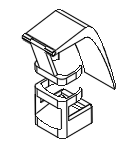
\includegraphics[width=3.25cm]{prototipo_arthropush.png}};

% Separador vertical
\draw[ArthroTeal!35, line width=0.8pt] (6.45,0.8) -- (6.45,8.2);

% ======================================================
% PANEL DERECHO GENERAL
% ======================================================
\fill[ArthroTeal!12, rounded corners=9pt] (6.85,0.75) rectangle (17.1,8.25);

% ======================================================
% TÍTULO PRINCIPAL
% ======================================================
\fill[white, rounded corners=7pt] (7.25,7.05) rectangle (16.7,8.0);

\node[
    text=ArthroNavy,
    font=\bfseries\large,
    align=center,
    text width=8.9cm
] at (11.98,7.52)
{ArthroPush};

% ======================================================
% BLOQUE INFORMACIÓN TÉCNICA
% ======================================================
\fill[white, rounded corners=7pt] (7.25,4.0) rectangle (12.35,6.75);

\node[
    anchor=north west,
    text=ArthroNavy,
    font=\bfseries\scriptsize,
    align=center,
    text width=4.55cm
] at (7.52,6.52)
{INFORMACIÓN TÉCNICA};

\node[
    anchor=north west,
    text=black,
    font=\fontsize{6.1}{7.0}\selectfont,
    align=left,
    text width=4.55cm
] at (7.50,6.15)
{\textbf{Modelo:} ARD-MDI-01\\
\textbf{Proyecto:} PR-PIB-GIS26-09\\
\textbf{Uso:} Adaptador para inhaladores MDI\\
\textbf{Material:} Polímero médico reciclable\\
\textbf{Función:} Ayuda a la pulsación manual\\
\textbf{Sin medicamento. No modifica dosis.}};

% ======================================================
% CÓDIGO DE BARRAS
% ======================================================
\fill[white, rounded corners=4pt] (7.55,2.72) rectangle (12.05,3.62);
\draw[black!20, rounded corners=4pt] (7.55,2.72) rectangle (12.05,3.62);

\foreach \x/\w in {
7.68/0.45,7.78/0.18,7.86/0.75,8.02/0.30,8.12/0.60,8.25/0.20,
8.36/0.95,8.52/0.35,8.64/0.70,8.78/0.20,8.90/0.85,9.05/0.30,
9.18/0.55,9.30/0.20,9.42/0.80,9.58/0.40,9.70/0.90,9.88/0.20,
10.00/0.50,10.12/0.25,10.25/0.95,10.44/0.35,10.57/0.70,
10.72/0.30,10.86/0.85,11.03/0.20,11.15/0.60,11.28/0.30,
11.40/0.95,11.58/0.40,11.72/0.75,11.88/0.20
}{
\draw[line width=\w mm] (\x,2.85) -- (\x,3.49);
}

\node[font=\fontsize{5.5}{6}\selectfont, text=black] at (9.8,2.53) {8 435672 091245};

% ======================================================
% BLOQUE ADVERTENCIAS
% ======================================================
\fill[white, rounded corners=7pt] (12.65,3.45) rectangle (16.7,6.75);

% Iconos advertencia más pequeños y separados del título
\draw[black!70, line width=0.35pt] (12.88,6.45) -- (13.03,6.68) -- (13.18,6.45) -- cycle;
\node[font=\tiny, text=black] at (13.03,6.51) {!};

\draw[black!70, line width=0.35pt] (16.17,6.45) -- (16.32,6.68) -- (16.47,6.45) -- cycle;
\node[font=\tiny, text=black] at (16.32,6.51) {!};

\node[
    text=ArthroNavy,
    font=\bfseries\scriptsize,
    align=center,
    text width=2.55cm
] at (14.56,6.0)
{ADVERTENCIAS\\DE USO};

\node[
    anchor=north west,
    text=black,
    font=\fontsize{5.15}{5.85}\selectfont,
    align=left,
    text width=3.45cm
] at (12.92,5.55)
{$\bullet$ Leer antes del uso.\\
$\bullet$ No usar si está dañado.\\
$\bullet$ Verificar ajuste estable.\\
$\bullet$ No forzar la palanca.\\
$\bullet$ Mantener fuera del alcance de niños.};

% ======================================================
% BLOQUE LIMPIEZA
% ======================================================
\fill[white, rounded corners=7pt] (7.25,1.22) rectangle (12.35,2.48);

\node[
    anchor=north west,
    text=ArthroNavy,
    font=\bfseries\scriptsize
] at (7.55,2.28)
{LIMPIEZA};

\node[
    anchor=north west,
    text=black,
    font=\fontsize{5.25}{5.9}\selectfont,
    align=left,
    text width=4.55cm
] at (7.55,2.00)
{Limpiar con paño húmedo y jabón neutro.\\
No usar disolventes ni abrasivos.\\
Conservar limpio, seco y protegido.};

% ======================================================
% BLOQUE INFORMACIÓN AMBIENTAL
% ======================================================
\fill[white, rounded corners=7pt] (12.65,1.35) rectangle (16.7,3.10);

\node[
    text=ArthroNavy,
    font=\bfseries\scriptsize,
    align=center,
    text width=3.5cm
] at (14.68,2.82)
{INFORMACIÓN\\AMBIENTAL};

\node[
    anchor=north west,
    text=black,
    font=\fontsize{5.35}{6.05}\selectfont,
    align=left,
    text width=3.45cm
] at (12.9,2.35)
{$\bullet$ Material reciclable.\\
$\bullet$ Separar del inhalador.\\
$\bullet$ Reciclar según normativa local.};

% Icono reciclaje sencillo
\node[text=ArthroTeal, font=\bfseries\small] at (16.28,2.82) {$\circlearrowleft$};

% ======================================================
% BLOQUE INFERIOR: TRAZABILIDAD + EMPRESA
% ======================================================
\fill[ArthroNavy!10, rounded corners=6pt] (7.25,0.50) rectangle (16.7,1.12);

\node[
    anchor=west,
    text=ArthroNavy,
    font=\fontsize{4.65}{5.2}\selectfont,
    align=left,
    text width=4.7cm
] at (7.45,0.83)
{\textbf{Fabricado por:} ArthroDesign Solutions S.L.\\
\textbf{Dirección:} Málaga, España};

\node[
    anchor=west,
    text=ArthroNavy,
    font=\fontsize{4.65}{5.2}\selectfont,
    align=left,
    text width=4.15cm
] at (11.75,0.83)
{\textbf{Email:} contacto@arthrodesign.com\\
\textbf{Lote:} LOT-XXXX};

\node[
    anchor=west,
    text=ArthroNavy,
    font=\fontsize{4.65}{5.2}\selectfont,
    align=left,
    text width=2.45cm
] at (15.05,0.83)
{\textbf{Fecha:} MM/AAAA\\
\textbf{Versión:} v1.0};

\end{tikzpicture}%
}
\caption{Diseño propuesto de la etiqueta exterior del embalaje.}
\end{figure}

\subsection{Simbología recomendada}

El etiquetado podrá incorporar símbolos gráficos sencillos para facilitar la comprensión por parte de usuarios mayores o con baja familiaridad técnica. La simbología propuesta se recoge en la Tabla 2.

\begin{table}[H]
\centering
\renewcommand{\arraystretch}{1.35}
\begin{tabularx}{\textwidth}{|p{4cm}|X|}
\hline
\rowcolor{ArthroNavy}
\textcolor{white}{\textbf{Símbolo / indicación}} & \textcolor{white}{\textbf{Significado}} \\
\hline
Leer instrucciones & El usuario debe consultar el manual antes del primer uso. \\
\hline
No usar si está dañado & El producto debe descartarse si presenta roturas, deformaciones o pérdida de ajuste. \\
\hline
No contiene medicamento & El adaptador es únicamente un accesorio mecánico y no incluye principio activo. \\
\hline
Producto reciclable & El material y el embalaje deben gestionarse conforme a las indicaciones locales de reciclaje. \\
\hline
Mantener limpio y seco & El producto debe conservarse en condiciones higiénicas y alejado de humedad excesiva. \\
\hline
\end{tabularx}
\caption{Simbología recomendada para el etiquetado del adaptador.}
\end{table}

\section{MANUAL DE INSTRUCCIONES}

\subsection{Contenido del embalaje}

Cada unidad comercial del adaptador ergonómico debe incluir los siguientes elementos:

\begin{itemize}
    \item Un cuerpo principal de sujeción para el inhalador MDI.
    \item Una palanca ergonómica de accionamiento.
    \item Un eje o elemento de articulación para el mecanismo de palanca.
    \item Una etiqueta exterior de identificación del producto.
    \item Un manual de instrucciones breve para el usuario.
\end{itemize}

Antes del primer uso, el usuario debe comprobar que todos los elementos están presentes, limpios y sin daños visibles.

\subsection{Uso previsto}

El adaptador está diseñado para reducir el esfuerzo necesario al presionar el cartucho de un inhalador MDI estándar. Su finalidad es facilitar la administración de la medicación en usuarios con dificultad para realizar el movimiento de pinza dactilar o para aplicar fuerza suficiente con los dedos.

El adaptador no debe utilizarse con inhaladores que no encajen de forma estable, que presenten una geometría incompatible o en los que el dispositivo bloquee la boquilla, la salida del aerosol o el correcto accionamiento del cartucho.

\subsection{Instrucciones de colocación}

\begin{enumerate}
    \item Compruebe que el inhalador MDI se encuentra limpio, seco y en buen estado.
    \item Introduzca el inhalador en el cuerpo principal del adaptador, manteniendo la boquilla libre y orientada hacia el exterior.
    \item Verifique que el cuerpo del adaptador queda ajustado alrededor del inhalador sin holguras excesivas.
    \item Sitúe la palanca sobre la parte superior del cartucho, de forma que el apoyo quede alineado con la zona de pulsación.
    \item Compruebe manualmente que la palanca se mueve de forma suave y que vuelve a su posición inicial sin atascarse.
\end{enumerate}

\subsection{Instrucciones de uso}

\begin{enumerate}
    \item Agite el inhalador si así lo indican las instrucciones del medicamento.
    \item Sujete el conjunto formado por inhalador y adaptador con una mano, asegurando un agarre estable.
    \item Coloque la boquilla del inhalador según las indicaciones del medicamento prescrito.
    \item Presione la palanca del adaptador con la palma o con el dedo que resulte más cómodo para el usuario.
    \item Coordine la pulsación con la inhalación siguiendo siempre las instrucciones del inhalador y la pauta indicada por el profesional sanitario.
    \item Tras la administración, retire el inhalador de la boca y compruebe que la palanca ha vuelto a su posición inicial.
\end{enumerate}

\subsection{Retirada del adaptador}

\begin{enumerate}
    \item Asegúrese de que el inhalador no está siendo accionado.
    \item Sujete el cuerpo principal del adaptador con una mano.
    \item Extraiga el inhalador suavemente, evitando forzar la palanca o deformar el cuerpo de sujeción.
    \item Guarde el adaptador en un lugar limpio, seco y protegido de golpes.
\end{enumerate}

\section{ADVERTENCIAS Y PRECAUCIONES}

Para garantizar un uso seguro del producto, deben respetarse las siguientes advertencias:

\begin{itemize}
    \item El adaptador no sustituye al inhalador ni modifica la medicación prescrita.
    \item El usuario debe seguir siempre las instrucciones del medicamento y las indicaciones del médico, farmacéutico o profesional sanitario.
    \item No utilizar el adaptador si presenta grietas, roturas, deformaciones, bordes cortantes o pérdida de estabilidad.
    \item No utilizar el producto si el inhalador queda suelto, inclinado o mal alineado.
    \item No forzar la palanca si el mecanismo ofrece resistencia anormal.
    \item No emplear el adaptador con inhaladores no compatibles o con formatos distintos a los MDI estándar.
    \item Mantener fuera del alcance de niños cuando no esté bajo supervisión de un adulto.
    \item No exponer el producto a temperaturas elevadas, fuentes directas de calor o productos químicos agresivos.
\end{itemize}

\section{LIMPIEZA Y MANTENIMIENTO}

\subsection{Limpieza ordinaria}

La limpieza debe realizarse de forma periódica, especialmente si el adaptador se utiliza diariamente. Para ello, se recomienda:

\begin{itemize}
    \item Limpiar la superficie exterior con un paño húmedo.
    \item Utilizar agua tibia y jabón neutro en caso de suciedad visible.
    \item Secar completamente el producto antes de volver a utilizarlo.
    \item Evitar la acumulación de polvo o restos en la zona de articulación de la palanca.
\end{itemize}

\subsection{Productos no recomendados}

No deben emplearse disolventes, lejía, alcohol concentrado, productos abrasivos ni herramientas punzantes para limpiar el adaptador, ya que podrían deteriorar el material, alterar el ajuste con el inhalador o generar bordes dañados.

\subsection{Revisión periódica}

Antes de cada uso, el usuario debe comprobar visualmente que el adaptador conserva su forma original, que la palanca se mueve correctamente y que no existen roturas o deformaciones. Si se detecta cualquier anomalía, el producto debe dejar de utilizarse y sustituirse por una nueva unidad.

\section{ALMACENAMIENTO Y CONSERVACIÓN}

El adaptador debe almacenarse en un lugar seco, limpio y protegido de impactos. Se recomienda conservarlo junto al inhalador o en su embalaje original para evitar pérdidas, suciedad o daños accidentales.

No debe guardarse bajo presión, doblado o en contacto con objetos pesados que puedan deformar la palanca o el cuerpo de sujeción. Tampoco debe exponerse de forma prolongada a radiación solar directa o temperaturas extremas.

\section{GESTIÓN AL FINAL DE LA VIDA ÚTIL}

Al final de su vida útil, el adaptador debe separarse del inhalador y gestionarse como residuo plástico reciclable siempre que las condiciones locales de reciclaje lo permitan. El embalaje exterior, si está fabricado en cartón, deberá depositarse en el contenedor correspondiente.

Si el adaptador ha estado en contacto con suciedad biológica o se encuentra deteriorado, deberá desecharse siguiendo las recomendaciones del centro sanitario, farmacia o normativa municipal aplicable.

\section{RESUMEN DE INFORMACIÓN PARA EL USUARIO}

\begin{table}[H]
\centering
\renewcommand{\arraystretch}{1.35}
\begin{tabularx}{\textwidth}{|p{4.2cm}|X|}
\hline
\rowcolor{ArthroNavy}
\textcolor{white}{\textbf{Aspecto}} & \textcolor{white}{\textbf{Indicación básica}} \\
\hline
Qué es & Accesorio mecánico para facilitar la pulsación de inhaladores MDI. \\
\hline
Para quién es & Usuarios con dificultad para presionar el cartucho del inhalador. \\
\hline
Cómo se usa & Se coloca sobre el inhalador y se presiona la palanca para accionar el cartucho. \\
\hline
Qué no hace & No contiene medicamento, no cambia la dosis y no sustituye instrucciones médicas. \\
\hline
Cuándo no usarlo & Si está roto, deformado, suelto o no encaja correctamente. \\
\hline
Cómo limpiarlo & Con paño húmedo, agua tibia y jabón neutro. \\
\hline
Cómo conservarlo & En lugar limpio, seco y protegido de golpes. \\
\hline
\end{tabularx}
\caption{Resumen de instrucciones esenciales para el usuario.}
\end{table}


% ======================================================
% BLOQUE DE FIRMAS
% ======================================================
\noindent\begin{minipage}{\textwidth}
    \begin{flushright}
        En Málaga, a \today
    \end{flushright}
    \vspace{2cm}

    \noindent
    \begin{minipage}[t]{0.45\textwidth}
        \centering
        \rule{6cm}{0.6pt} \\
        \textbf{Fdo. D. Sergio Carmona Muñoz} \\
        Colegiado Nº 06424 \\
        DNI: 26291930D
    \end{minipage}
    \hfill
    \begin{minipage}[t]{0.45\textwidth}
        \centering
        \rule{6cm}{0.6pt} \\
        \textbf{Fdo. D. Juan Gabriel Navarro Valdivielso} \\
        Colegiado Nº 06425 \\
        DNI: 77666662D
    \end{minipage}

    \vspace{2cm}

    \noindent
    \begin{minipage}[t]{0.45\textwidth}
        \centering
        \rule{6cm}{0.6pt} \\
        \textbf{Fdo. D. Antonio Sánchez Doña} \\
        Colegiado Nº 06423 \\
        DNI: 79380534J
    \end{minipage}
    \hfill
    \begin{minipage}[t]{0.45\textwidth}
        \centering
        \rule{6cm}{0.6pt} \\
        \textbf{Fdo. D. Iván de la Torre Segato} \\
        Colegiado Nº 06421 \\
        DNI: 79383630G
    \end{minipage}
\end{minipage}
\vspace{1cm}

% ======================================================
% HOJA EN BLANCO CON MARCA DE AGUA
% ======================================================
\newpage
\pagestyle{fancy}

\begin{tikzpicture}[remember picture, overlay]
    \node[opacity=0.1] at (current page.center) {
\includegraphics[width=12cm]{logo_definitivo.png}};
\end{tikzpicture}

% Empujamos el texto hacia la parte inferior del folio
\vspace*{8.5cm} 
\begin{center}
    \textit{Esta hoja ha sido dejada deliberadamente en blanco.}
\end{center}
\vfill

\end{document}